\subsection{Modes in TEM Cells}\label{sec:modes_tem_cell}
\subsubsection{Power transfer of modes}
% Goal is to describe the modes in a TEM cell, including their cut-off frequencies. \cite{Kreindl_Bauernfeind_Weiss_Stockreitner_Kaltenbacher_2024} shows that these investigations are important. There are also modes propagating perpendicular to the intended propagation direction. Why are no waveguides used? Explain.

% In this paper, a VCSEL with a decoupling capacitor are modeled. It is visible, that the electric coupling dominates at an orientation of 90°. A local minimum is then visible. At 400\,MHz and upwards, inductive coupling becomes dominant, but only at 0° where it couples with the septum. It is possible, that a certain mode can propagate at a certain frequency, which influenced the result in this paper. 


Any electromagnetic field distribution in a waveguide can be represented by an infinite series of normal modes. \autoref{eqn:norm_power} shows that each mode is orthogonal to each other, with $\mathbf{e_n}^\pm$ and $\mathbf{h_n^\pm}$ being the function vectors of the electric and magnetic field in transverse direction \cite{Collin_2015}. A coupling between the modes only occurs due to geometric changes of the waveguide. Additionally, each mode is normalized to $\sqrt{\mathrm{W}}$, shown by \autoref{eqn:unit_power}. Only the transverse fields are investigated in these Equations, because they carry power along the waveguide, opposed to the fields in the propagation direction.

\begin{align}
    \iint \mathbf{e_n^\pm}\times \mathbf{h_m^\pm}\mathrm{d}S\mathbf{n}&=0 \quad\text{if}\quad n\neq m
    \label{eqn:norm_power}\\
    \iint \mathbf{e_n^\pm}\times \mathbf{h_n^\pm}\mathrm{d}S\mathbf{n}&=1
    \label{eqn:unit_power}
\end{align}

The radiated fields can be described by a summation of normal modes, as in \autoref{eqn:modal_superposition1} and \autoref{eqn:modal_superposition2}. The coefficients of these modes are straightforward to calculate, due to Lorentz Reciprocity Theorem, if the waveguide's walls are perfectly conducting. Ideally, any higher order mode than the first TEM mode will be suppressed, and the calculation simplifies to $n=0$. Additionally, it is assumed that the source is electrically small, which makes it possible to represent it with dipoles, further simplifying the equations \cite{Koepke_1989}. 

\begin{align}
    \mathbf{E^\pm}&=\sum_na_n\mathbf{E_n^\pm}    \label{eqn:modal_superposition1}\\
    \mathbf{H^\pm}&=\sum_na_n\mathbf{H_n^\pm}    \label{eqn:modal_superposition2}
\end{align}

Suppose a current source $\mathbf{J_1}$ excites a waveguide (as is the case with the dipoles in the TEM cell). Normally, such a current source would be driven with external fields, but for the sake of the argument, they are ignored. Only $\mathbf{E}$ and $\mathbf{H}$ are considered, which are the fields radiated by $\mathbf{J_1}$. Additionally, $\mathbf{E}_n^\pm$ and $\mathbf{H}_n^\pm$ are the resulting waveguide fields, with the signs indicating the direction of propagation. Take \autoref{eqn:lorentz_rec_theorem_int} and set $\mathbf{J_2}=\mathbf{M_1}=\mathbf{M_2}=0$. Now, only the current source $\mathbf{J_1}$ remains, and the \autoref{eqn:J1_propagating_waves} emerges. % Explain how certain surfaces do not to have be integrated, therefore rendering this equation very useful. Also, the expansion coefficients can be determined. Maybe do this calculation with a rectangular waveguide.

\begin{equation}
    \oiint _S (\mathbf{E_n^\pm}\times \mathbf{H}-\mathbf{E}\times \mathbf{H}_n^\pm)\cdot\mathrm{d}\mathbf{S}=\iiint \mathbf{J_1}\cdot\mathbf{E_n^\pm}\mathrm{d}V
    \label{eqn:J1_propagating_waves}
\end{equation}

\begin{figure}[t]
	\centering
	\includegraphics[width=0.7\linewidth]{content/img/reciprocity_tem_cell}
	\caption{TEM cell with an arbitrary current source $\mathbf{J}$ along the curve $\mathbf{\tau}$. $\mathbf{E}$ and $\mathbf{H}$ are the field intensities induced by the current. $\mathbf{E}^+$ and $\mathbf{E}^-$ are outgoing fields towards both output ports of the TEM cell. $\mathbf{S}$ indicates the surface, and $V$ the volume of the domain in question.}
	\label{fig:reciprocitytemcell}
\end{figure}


In case of the TEM cell, it is desirable that only the TEM mode is propagating, and that the source is represented by a dipole. When the expansions \autoref{eqn:modal_superposition1}, \autoref{eqn:modal_superposition2} and the orthogonal property \autoref{eqn:norm_power} are used, and when considering an electric dipole, the \autoref{eqn:dipole_tem_waves} arises. In this equation, the wave amplitudes $a$ and $b$ are given through the surface integral in the Lorentz Reciprocity theorem, with $a$ being the wave going to the left side, and $b$ to the other. The electric dipole moment $\mathbf{m_e}$ is given by the current $\mathbf{J}$ flowing through the infinitesimal wire. Note that only the electric field of TEM wave propagation is considered. In reality, more modes may propagate, for which the electric field must be replaced by the superposition of normal modes as in \autoref{eqn:modal_superposition1}. %Additionally, to calculate the exact value of the electric field, a series of image sources as a Green's function may be applied.

\begin{equation}
\begin{pmatrix}a \\b\end{pmatrix} = -\frac{1}{2}\mathbf{m_e}\cdot \mathbf{E}^\pm
\label{eqn:dipole_tem_waves}
\end{equation}
\todo{$E_n^\pm$?}

If this arbitrary current distribution forms an infinitesimal loop, the source can be represented by a magnetic dipole moment $\mathbf{m_m}$. It is defined by the product $\mathbf{m_m}=\mathbf{A}\cdot I$, an infinitesimal current loop with area $A$ carrying a current $I$. This leads to \autoref{eqn:mag_dipole_moment_tem}. This formulation assumes, that the magnetic field strength $\mathbf{H}^\pm$ does not change over the loop area, i.e. the loop is electrically small. Otherwise, the magnetic field strength $\mathbf{H}^\pm$ must be considered in the integration \cite{Collin_2015,Sreenivasiah_Chang_Ma_1981}.

\begin{align}
    \begin{pmatrix}a \\b\end{pmatrix} &= -\oint_C \mathbf{E}^\pm \mathrm{d}l \nonumber \\
    &= -\iint_{S_0} \nabla \times \mathbf{E}^\pm \mathrm{d}\mathbf{S}\nonumber\\
    &= \mathrm{i}\omega\mu_0\iint_{S_0} \mathbf{H}^\pm\cdot \mathrm{d}\mathbf{S}\nonumber\\
    &= \mathrm{i}\omega\mu_0\mathbf{m}_m\mathbf{H}^\pm 
    \label{eqn:mag_dipole_moment_tem}
\end{align}


If there are several modes propagating, it is useful to find the coefficients of the modes $a_n$ and $b_n$ in \autoref{eqn:modal_superposition1} and \autoref{eqn:modal_superposition2}. In this case, the orthogonality property in \autoref{eqn:norm_power} is used to derive \autoref{eqn:an} and \autoref{eqn:bn} \cite{Collin_2015}. The wire is described by a curve C, and the tangential vector $\boldsymbol{\tau}$ is used to integrate along this curve.

\begin{subequations}
    \begin{equation}
        2a_n = -\int_C \boldsymbol{\tau}\cdot\mathbf{E}_n^-\mathrm{d}l
        \label{eqn:an}
    \end{equation}
        \begin{equation}
        2b_n = \int_C \boldsymbol{\tau}\cdot\mathbf{E}_n^+\mathrm{d}l
        \label{eqn:bn}
    \end{equation}
\end{subequations}

\subsubsection{Modes in rectangular waveguides}

A TEM cell is used for EMC test specifications. It makes the conduction of TEM waves possible, which resemble planar free-space waves. Additionally, it shields the waves from radiating to the sides, for which it has a clear advantage to a stripline \cite{809846,990711}. A simple rectangular waveguide cannot be used for this application. Assuming that a monochromatic wave travels down the waveguide, the waves will propagate without dampening only at a certain angle of reflection on the perfectly conducting surface. A short mathematical proof can be shown here, using Maxwell's equation. It shows that the electric and magnetic fields in direction of propagation cannot both be zero. 
\begin{align}
    \mathbf{E}&=(E_{0,x}\cdot\mathbf{e_x}+E_{0,y}\cdot\mathbf{e_y}+E_{0,z}\cdot\mathbf{e_z})\mathrm{e}^{\mathrm{i}(\omega t-kz)}\\
    \mathbf{H}&=(H_{0,x}\cdot\mathbf{e_x}+H_{0,y}\cdot\mathbf{e_y}+H_{0,z}\cdot\mathbf{e_z})\mathrm{e}^{\mathrm{i}(\omega t-kz)}\\
    \nabla \times \mathbf{E} &=\begin{pmatrix}\frac{\mathrm{d}}{\mathrm{d}y}E_z-\mathrm{i}kE_y \\\mathrm{i}kE_x-\frac{\mathrm{d}}{\mathrm{d}x}E_z \\\frac{\mathrm{d}}{\mathrm{d}x}E_y-\frac{\mathrm{d}}{\mathrm{d}y}E_x\end{pmatrix}=\begin{pmatrix} -\mathrm{i}\omega B_x\\-\mathrm{i}\omega B_y\\ -\mathrm{i}\omega B_z \end{pmatrix}\\
    \nabla \times \mathbf{B} &=\begin{pmatrix}\frac{\mathrm{d}}{\mathrm{d}y}B_z-\mathrm{i}kB_y \\\mathrm{i}kB_x-\frac{\mathrm{d}}{\mathrm{d}x}B_z \\\frac{\mathrm{d}}{\mathrm{d}x}B_y-\frac{\mathrm{d}}{\mathrm{d}y}B_x\end{pmatrix}=\begin{pmatrix} \frac{\mathrm{i}\omega}{\mu\epsilon} E_x\\\frac{\mathrm{i}\omega}{\mu\epsilon} E_y\\ \frac{\mathrm{i}\omega}{\mu\epsilon} E_z \end{pmatrix}
\end{align}

If $E_z$ and $B_z$, the fields in direction of propagation, were both zero, then the change of the transverse fields would be constantly zero, and because of the boundary conditions, all transverse fields would be zero. \autoref{eqn:rect_waveguide_gauss} shows Gauss' law and \autoref{eqn:rect_waveguide_faraday} Faraday's law if $E_z=B_z=0$, from which the unchanging transverse electric field can be derived. 

\begin{align}
    \frac{\mathrm{d}}{\mathrm{d}x}E_x+\frac{\mathrm{d}}{\mathrm{d}y}E_y&=0\quad\text{Derived out of Gauss' law}\label{eqn:rect_waveguide_gauss}\\
    \frac{\mathrm{d}}{\mathrm{d}y}E_x-\frac{\mathrm{d}}{\mathrm{d}x}E_y&=0\quad\text{Derived out of Faraday's law}\label{eqn:rect_waveguide_faraday}
\end{align}

\subsubsection{TEM Mode in TEM Cells}

A TEM cell solves this problem, by having a gap between the septum and the side walls. Essentially, it can be considered as two rectangular waveguides with apertures on the sides. Those apertures allow perturbations of the electromagnetic fields between them. The boundary conditions of the Laplace equation now changed due to the gaps. The Green's function may be calculated of the new construction, now considering the boundary conditions at the gaps, which must be the same for both waveguides (to prevent discontinuities). In the papers of Tippet, Chang and Wilson, this new Green's function lead to the excitation of TEM modes in both waveguides \cite{Tippet_Chang_Crawford_1976,Wilson_1981}. However, the gap is assumed to be small, electrically ($\xi g \ll 1$) and compared to the septum width ($g/a \ll 1$) \cite{4091747}. The variable $\xi=\sqrt{k_0^2 - \beta ^2}$ is the transverse (in y-direction) propagation constant, and consists of the free-space wave number $k_0$ and longitudinal (in z-direction) propagation constant $\beta$. The variables $g$ and $a$ are geometry variables of the TEM cell annotated in \autoref{fig:verticalantennatemcell}.

\begin{figure}[h]
	\centering
	\includegraphics[width=0.7\linewidth]{content/img/vertical_antenna_tem_cell}
	\caption{TEM cell with vertical antenna inserted}
	\label{fig:verticalantennatemcell}
\end{figure}


To analyze the fields in a TEM cell, the dyadic Green's function discussed in \autoref{sec:dyad_green} proofs itself to be useful. It is assumed, that a vertical, electrically short antenna is inserted in the top center of the TEM cell. This is modeled by a current distribution in y-direction $\mathbf{\hat J}(\mathbf{x}) = \mathbf{a}_y J(\mathbf{x})$ \cite{4091747}. Accordingly, the Green's function reduces to $\mathbf{\hat G}(\mathbf{x, x'}) = \mathbf{a}_y G(\mathbf{x, x'})$. \todo{Check Vector notation. Is correct for Dyadics?} First, the Green's function for a rectangular waveguide $G_O(\mathbf{x,x'})$ is shown in \autoref{eqn:unperturbed_green} \cite{Balanis_1997}. There, $\eta_0$ is the free-space impedance, $M=m\pi / (2a)$, $N=n\pi/b$ and $K_m=(\xi^2-M^2)^{1/2}$. Furthermore,

$\Delta_n = 
\begin{cases}
	\frac{1}{2}, & n = 0 \\
	1,           & n > 0
\end{cases} $ 

and,

$g_{mn}(\mathbf{x}_t, \mathbf{x}_t') = \left( \frac{2}{ab} \right)
\sin M(x + a) \sin M(x' + a)
\cdot \cos Ny \cos Ny'$

are functions implemented in \autoref{eqn:unperturbed_green}. The components $x$, $x'$ and $y$, $y'$ are part of the vectors $\mathbf{x}_t$, $\mathbf{x}'_t$. 

\begin{equation}\label{eqn:unperturbed_green}
	\tilde{G}_0(\mathbf{x}_t, \mathbf{x}_t') =
	\frac{-\mathrm{j} \eta_0}{k_0} \left\{\sum_{m,n=0}^{\infty} \frac{\Delta_n [M^2 + \beta^2]}{M^2 + N^2 - \xi^2} \; g_{mn}(\mathbf{x}_t, \mathbf{x}_t')
	\right\}
\end{equation}


The TEM cells Green's function by adding a unperturbed term to it \cite{4091747}. The derivation of those Green's Functions is demonstrated in \cite{Wilson_1981}, which uses the same methods described in \cite{Balanis_1997}, as mentioned above.

The perturbed term in \autoref{eqn:perturbed_green} describes the influence of the gaps on the field distribution. They are derived by forcing the tangential fields to be continuous across the gaps, then describing this boundary condition mathematically as a perturbing second Green's function. The rest of the boundary conditions on the are zero due to the geometry of the TEM cell. The functions used are,

\begin{equation*}
L(\beta) = \left[
\ln \left( \frac{8a}{\pi g} \right)
- \frac{\pi}{a} \sum_{m \in \{1,3,5,...\}}^{\infty} \left(
\frac{\cot K_m b}{K_m}
+ \frac{2a}{m\pi}
\right)
\right]^{-1}
\end{equation*}

and, 

\begin{equation*}
f(\mathbf{x}_t) = \sum_{m \in \{1,3,5,...\}}^{\infty} M \frac{\cos K_{m} (b - y)}{K_{m} \sin K_{m} b}
\sin Ma \cos Mx J_0(Mg).
\end{equation*}

To receive the final Green's Function, the unperturbed and perturbed term are added together ${G}(\mathbf{x}_t, \mathbf{x}'_t) = {G}_O(\mathbf{x}_t, \mathbf{x}'_t)+{G}_g(\mathbf{x}_t, \mathbf{x}'_t)$. Naturally, the observation point $\mathbf{x}$ can only be on the upper half in the chamber, where the source is also located \cite{4091747}. 


\begin{equation}\label{eqn:perturbed_green}
	\widetilde{G}_g(\mathbf{x}_t, \mathbf{x}'_t) = \frac{ -j \pi k_0 \eta_0}{2 a^2 s^2} L(\beta) f(\mathbf{x}_t) f(\mathbf{x}'_t)
\end{equation}

Because waves propagating in the TEM cell are assumed to travel into infinity, they might have any longitudinal propagation constant $\beta$. They are not limited by boundary conditions in this direction. It therefore proofs useful to apply a Fourier Series over this variable, as done in \autoref{eqn:greens_fourier}. There, the subscript $t$ indicates only the transverse (xy-plane). 
\todo{This explanation is not directly cited but my interpretation. Make sure that this is correct info.}

\begin{subequations}\label{eqn:greens_fourier}
	\begin{equation}
	G_O(\mathbf{x,x'})=\frac{1}{2\pi}\int^\infty_{-\infty} \tilde{G}_0(\mathbf{x_t,x_t'})\mathrm{e}^{j\beta z}\mathrm{d}\beta
	\end{equation}
	\begin{equation}
	G_g(\mathbf{x,x'})=\frac{1}{2\pi}\int^\infty_{-\infty} \tilde{G}_g(\mathbf{x_t,x_t'})\mathrm{e}^{j\beta z}\mathrm{d}\beta
	\end{equation}
\end{subequations}



Now, the antenna impedance is calculated using the generic \autoref{eqn:antenna_imp}. The Green's Function in this represents the electric field excited by an unit strength dipole \cite{4091747}. Scaled by multiplication with the current density  $\mathbf{J}(\mathbf{x})$ and integrated over the length of the wire, results in the total electric field. Next, by multiplying it by the current distribution $\mathbf{J}(\mathbf{x})$ and integrated over the length of the wire again, leads to the apparent power. In the end, dividing this term by the total current consumption squared $I^2$ leads to the impedance.


\begin{equation}\label{eqn:antenna_imp}
	Z = \frac{-1}{I^2} \int_S \int_{S'} \mathbf{J}(\mathbf{x}) \cdot \mathbf{G}(\mathbf{x}, \mathbf{x}') \cdot \mathbf{J}(\mathbf{x}') \, \mathrm{d}s' \, \mathrm{d}s
\end{equation}

When evaluating the real part of the impedance for the case described here, the radiation resistance results from \autoref{eqn:rad_res}. If the inserted antenna is electrically small, as it is in this case, $d$ reduces the influence of other terms. The most dominant term then, $k_0^2$, results in a quadratic relation of the radiation resistance to the frequency. This agrees with the theoretical framework in the discussion about small dipoles in \autoref{sec:dipoles}, as well as with the simulations results in \autoref{sec:simulations}.

\begin{equation}\label{eqn:rad_res}
	R = \frac{ \pi \eta_0 k_0^2 }{ 4 a^2 } \csc^2{ k_0 d } \, L(k_0) H(k_0)
\end{equation}

Here, 
\begin{equation*}
H(\beta) = \sum_{m' \in \{1,3,5,...\}}^{\infty} h_{m'}(\beta) \sum_{m \in \{1,3,5,...\}}^{\infty} h_m(\beta) J_0(r(M^2 + \beta^2)^{1/2})
\end{equation*}

and,

\begin{equation*}
h_m(\beta) = \frac{M \sin Ma J_0(Mg)}{K_m \sin K_m b} \cdot 
\frac{\cos k_0 d - \cos K_m d}{M^2 + \beta^2}.
\end{equation*}

\todo[inline]{Give a short interpretation of each variable. Subdivide the text into subsections}

% To do this, the electric and magnetic field are described by the wave equations in \autoref{eqn:wave_equ_e_field} and \autoref{eqn:wave_equ_h_field} \cite{Collin_2015}. 

% \begin{subequations}
% \begin{equation}
%     \left(\nabla^2-\mu\epsilon\frac{\mathrm{d^2}}{\mathrm{d}t^2}\right)\mathbf{E}(\mathbf{x})=\mu\frac{\mathrm{d}}{\mathrm{d}t}\mathbf{J}+\frac{\nabla\rho}{\epsilon}
%     \label{eqn:wave_equ_e_field}
% \end{equation}

% \begin{equation}
%     \left(\nabla^2-\mu\epsilon\frac{\mathrm{d^2}}{\mathrm{d}t^2}\right)\mathbf{H}(\mathbf{x})=-\nabla\times\mathbf{J}
%     \label{eqn:wave_equ_h_field}
% \end{equation}
% \end{subequations}

% The Green's function must solve these wave equations, therefore it is formulated as \autoref{eqn:greens_function_wave_equ}. The boundary condition for the Green's function is $\frac{\mathrm{d}}{\mathrm{d}\mathbf{n}}\mathbf{G}=0$, which sets the normal derivative at the boundary to zero. ACHTUNG: ICH GLAUBE, DASS DAS NUR IM FALL \cite{Wilson_1981} FUNKTIONIERT, IN WELCHEM NUR DIE Z KOMPONENTEN BEACHTET WERDEN. DIESE ÄNDERN SICH NICHT ÜBER DIE GAP. This boundary condition applies everywhere, meaning to every conducting surface, as well as the gaps between the septum and the walls of the TEM cell. Consequently, any discontinuities in fields are prevented.

% \begin{equation}
%     \left(\nabla^2-\mu\epsilon\frac{\mathrm{d^2}}{\mathrm{d}t^2}\right)\mathbf{G}(\mathbf{x}-\mathbf{x'})=-\delta(\mathbf{x}-\mathbf{x'})
%     \label{eqn:greens_function_wave_equ}
% \end{equation}

% The solution to this given problem has been solved before \cite{Collin_2015}. Here, the TE guide mode expansion in \autoref{eqn:greens_function_rect_waveguide_solved} are included \cite{Wilson_1981}. THIS IS ONLY Z-COMPONENT OF FIELDS! THERE IS NO VECTOR.

% \begin{equation}
%     \mathbf{G}(\mathbf{x}-\mathbf{x'})=\left(\frac{2}{ab}\right)\sum^\infty_{m,n=0}\frac{\Delta_m\Delta_n}{(K^2_{mn}-k^2)}\cos{\left( \frac{m\pi}{2a}(x+a) \right)}\cos{\left( \frac{m\pi}{2a}(x'+a) \right)}\cos{\left( \frac{n\pi y}{b}\right)}\cos{\left( \frac{n\pi y'}{b}\right)}
%     \label{eqn:greens_function_rect_waveguide_solved}
% \end{equation}

% \begin{itemize}
%     \item $\mathbf{x}$ is the observation point
%     \item $\mathbf{x'}$ is the source point
%     \item $a$ and $b$ are the height and width of the rectangular waveguide
%     \item $m, n$ are the indices of the TE mode
%     \item $x$ is the x-component of the observation point $\mathbf{x}$
%     \item $y$ is the y-component of the observation point $\mathbf{x}$
%     \item $x'$ is the x-component of the source point $\mathbf{x}$
%     \item $y'$ is the y-component of the source point $\mathbf{x}$
%     \item $K_{mn} = \left[ \left( \frac{m\pi}{2a} \right)^2+\left( \frac{n\pi}{b} \right)^2 \right]^{1/2}$
%     \item $k$ is the wave number $\frac{2\pi}{\lambda}$
%     \item $\Delta_m=\begin{cases}1/2, & \text{if } m = 0 \\1,       & \text{if } m \neq 0\end{cases}$ and $\Delta_n=\begin{cases}1/2, & \text{if } n = 0 \\1,       & \text{if } n \neq 0\end{cases}$
% \end{itemize}

% To use the Green's function to solve the magnetic fields, \autoref{eqn:wave_equ_h_field} is multiplied with the Green's function $\mathbf{G}(\mathbf{x}-\mathbf{x'})$, and \autoref{eqn:greens_function_wave_equ} with the magnetic field $\mathbf{H}(\mathbf{x})$. The two resulting equations are subtracted from each other, which leads to \autoref{}.

% \begin{equation}
%     \mathbf{G}(\mathbf{x}-\mathbf{x'})\frac{\mathrm{d^2}}{\mathrm{d}t^2}\mathbf{H}(\mathbf{x})-\mathbf{H}(\mathbf{x})\frac{\mathrm{d^2}}{\mathrm{d}t^2}\mathbf{G}(\mathbf{x}-\mathbf{x'})=-\mathbf{G}(\mathbf{x}-\mathbf{x'})\nabla\times\mathbf{J}(\mathbf{x})+\mathbf{H}(
% \end{equation}

\subsubsection{Higher order modes in TEM cells}

The TEM cell used in the simulation has a width of $a=40\,\mathrm{mm}$ and a height of $b=24\,\mathrm{mm}$. A cross section of the TEM cell with the important dimensions is shown in \autoref{fig:tem_cell_crosssection}. The cutoff frequencies of the higher order TE and TM modes can be approximated by the same formula, shown in \autoref{eqn:cutoff_frequency_rect_waveguide} for rectangular waveguides. However, this is only true, if the septum is very thin ($t/b \ll 0.1$), and for modes with n-even subscripts, i.e. TE\textsubscript{m,2n} and TM\textsubscript{m,2n} modes.

\begin{figure}[h]
    \centering
    \includegraphics[width=0.5\linewidth]{content/img/tem_cell_crosssection.png}
    \caption{Cross section of the TEM cell}
    \label{fig:tem_cell_crosssection}
\end{figure}

\begin{equation}
    f_c = \frac{c}{2} \sqrt{\left(\frac{m}{a}\right)^2 + \left(\frac{n}{b}\right)^2}
    \label{eqn:cutoff_frequency_rect_waveguide}
\end{equation}

\begin{itemize}
  \item \( f_c \): cutoff frequency of the mode \(\text{T}_{mn}\)
  \item \( c \): speed of light in the medium (approximately \(3 \times 10^8 \, \text{m/s}\) in air)
  \item \( a \): wider dimension (broad wall) of the rectangular waveguide (meters)
  \item \( b \): narrower dimension (narrow wall) of the rectangular waveguide (meters)
  \item \( m \): mode index in the \(a\)-direction (integer, \(m \geq 0\))
  \item \( n \): mode index in the \(b\)-direction (integer, \(n \geq 0\))
\end{itemize}

The cutoff frequency of the TE\textsubscript{10} mode is around 3.75\,GHz, according to \autoref{eqn:cutoff_frequency_rect_waveguide}. To verify this, a modal analysis was performed in Ansys HFSS, where an empty TEM cell was modeled with two waveports defined at its output. The resulting S\textsubscript{12}-parameters are presented in\autoref{fig:te01_te10_tem_propagation}. The black line shows the S\textsubscript{12}-parameter over the frequency of the TEM mode, while the blue line demonstrates S\textsubscript{12}-parameter of the TE\textsubscript{10} mode. At a frequency of 3.75\,GHz, the mode propagates without attenuation, where the cutoff frequency $f_\mathrm{c,10}$ is defined. The simulated result comes very close to the analytically determined one. 

The red trace shows a cutoff frequency of $f_\mathrm{c,10}=3.12\,\mathrm{GHz}$ for the TE\textsubscript{01} mode. \autoref{eqn:cutoff_frequency_rect_waveguide} would predict a cutoff frequency of 6.25\,GHz, however, the septum influences n-odd modes like this one. Their cutoff frequencies are shifted to a lower value \cite{Weil_Gruner_1984}. 

The frequency in simulations with the TEM cell will range from 1\,MHz to 3\,GHz. This guarantees that the higher order modes will not influence the simulation results.

%The first TM mode would be the TM\textsubscript{11} mode, since TM\textsubscript{01} and TM\textsubscript{10} do not exist.

In a real TEM cell, a tapered section transform the TEM waveguide to a coaxial transmission line. This section does not cause reflections of waves in TEM mode. However, higher order TE and TM modes get reflected, and because the TEM cell is a high-Q cavity, resonances occur at $\frac{\lambda}{4}$ or $\frac{\lambda}{2}$ \cite{990711}. This is not considered in these simulations, since the simulation model does not contain this tapered section. \todo{Maybe do simulations with such a tapered section. See \cite{990711}}

% \autoref{tab:even_n_modes} shows the cutoff frequencies of the n-even modes. The cutoff frequencies of the n-odd modes either have to be determined by the approximation in \cite{Wilson_Ma_1986} or analyzed numerically. \todo{Do either one of these}


% \begin{table}[h]
%     \centering
%     \begin{tabular}{ccc}
%         Mode & Calculated $f_c$ & Measured $f_c$\\
%         TE\textsubscript{10} & 750\,MHz & \\
%         TE\textsubscript{20} & 1.50\,GHz & \\
%         TE\textsubscript{12} & 3.09\,GHz & \\
%         TM\textsubscript{20} & 1.50\,GHz & \\
%         TM\textsubscript{12} & 3.09\,GHz & \\
%     \end{tabular}
%     \caption{Caption}
%     \label{tab:even_n_modes}
% \end{table}

\begin{figure}[h]
    \centering
    \includegraphics[width=1\linewidth]{content/img/tem_cell_modes.png}
    \caption{Propagation of TEM, TE\textsubscript{01} and TE\textsubscript{10} modes in TEM cell}
    \label{fig:te01_te10_tem_propagation}
\end{figure}




The TEM cell does not only support TEM modes, above their cut-off frequency TE and TM modes begin to propagate. Because the TEM cell is a high-Q cavity, those cut-off frequencies are sharply defined frequencies. Due to imperfections, change in materials or finite conductivity of the conducting plates, wave propagating in the TEM mode may excite higher order TE and TM modes, too \cite{10791592}. A change in material, for example, demands the electric and magnetic field to have a component in the direction of propagation at the discontinuity. A paper by Wilson and Ma present analytical approximations to determine these frequencies \cite{Wilson_Ma_1986}.  There is a long list for the several first few corner frequencies of the first modes. Additionally, a paper by Koch, Groh and Garbe determines the resonance frequencies of the first TE modes analytically \cite{10791592}. The TEM mode is necessarily excited by the geometry of the TEM cell, hence this mode is called essential. The higher order TE and TM modes, which are only excited due to non-uniformity of the TEM cell, are called non-essential modes \cite{990711}.


The first modes propagating after the TEM mode is the TE\textsubscript{10} and TE\textsubscript{01} modes. Their transversal electric fields are depicted in \autoref{fig:transversal_e_fields_tem_cell}. 

\begin{figure}[h]
    \centering
    \begin{subfigure}[b]{0.3\linewidth}
        \centering
        \includegraphics[width=\linewidth]{content/img/tem_cell_mode.png}
        \caption{TEM Mode}
        \label{fig:tem_mode}
    \end{subfigure}
    \begin{subfigure}[b]{0.3\linewidth}
        \centering
        \includegraphics[width=\linewidth]{content/img/te01_mode.png}
        \caption{TE\textsubscript{01}}
        \label{fig:te01_mode}
    \end{subfigure}
    \begin{subfigure}[b]{0.3\linewidth}
        \centering
        \includegraphics[width=\linewidth]{content/img/te10_mode.png}
        \caption{TE\textsubscript{10}}
        \label{fig:te10_mode}
    \end{subfigure}
    \caption{Transversal electric fields in cross section of TEM cell}
    \label{fig:transversal_e_fields_tem_cell}
\end{figure}
\todo{Vector directions are wrong in the pictures. Additionally, update cutoff frequencies.}

The cut-off frequencies are dependent on the dimensions of the TEM cell, as previously shown. \autoref{tab:modes_tem_cell} shows some cut-off frequencies of these modes for different TEM cell dimensions. The TE\textsubscript{10}-mode is independent of the height $b$ of the TEM cell, as would be the case in a rectangular waveguide. Both the TE\textsubscript{10}-mode and the TE\textsubscript{01}-mode are dependent on the width $a$. Note that a port impedance of $50\,\Omega$ is only kept in the case $a=40\,\mathrm{mm}$ and $b=24\,\mathrm{mm}$. This information is important when varying the TEM cell dimension, as is done when investigating near-field ($k\cdot r < 1$) and intermediate-field ($k\cdot r = 1$) coupling. 

\begin{table}[h]
\centering
\caption{Cut-off frequencies of higher order modes depending on TEM cell dimensions}
\label{tab:modes_tem_cell}
\begin{tabular}{|c|c||c|c|}
	\hline
	a [mm]& b [mm]&TE\textsubscript{01} $f_c$ [GHz] &TE\textsubscript{10} $f_c$ [GHz]\\
	\hline\hline
	80 & 24 & 1.89 & 2.05 \\
	\hline\hline
	40 & 24 & 3.17 & 3.76 \\
	\hline\hline
	40 & 48 & 2.10 & 3.76 \\
	\hline
\end{tabular}
\end{table}





